\section{附錄二、輸入/輸出 (Input/Output, I/O)}
基本上,\cc{}語言涵括了C語言的功能,所以我們也可以在\cc{}的環境中,撰寫C的程式碼。一般而言,大部份的程式都會有輸入和輸出的需求,而\cc{}和C的輸入和輸出方式,各有其優點,在不同的場合,有時候使用\cc{}的輸入輸出方式會比較方便,有時候使用C的輸入輸出函數會比較方便,如果可以把兩種方式都學會,在撰寫程式碼的時候,可以有很多便利,所以這裡先介紹兩種語言基本的輸入和輸出的使用方法。

\subsection{C語言的輸入和輸出}
C語言使用scanf和printf兩個函數來做輸入和輸出,使用C語言的輸入輸出函數,C程式碼必須引入檔頭<stdio.h>,如果在\cc{}的環境中,則可以引入<stdio.h>或<cstdio>。以下先介紹printf函數的用法,接著再介紹scanf函數的用法。

\subsubsection {printf輸出函數}
C語言使用printf函數將訊息列印至標準輸出(standard output),一般而言,標準輸出指的是螢幕,除了列印字串,也可以列印各種型態的變數,執行過後會回傳所列印的字元數。printf函數至少要有一個參數,而且第一個參數一定是一個字串,執行結果會把這個字串列印到螢幕上,例如:
\begin{inside}
	printf("format string");
\end{inside}
其執行結果如下:
\begin{Verbatim}
    format string
\end{Verbatim}
字串中可以加入跳脫符號,用來控制輸出的樣貌,常用的控制字元如\autoref{escapechar}所示,例如
$\backslash$n代表換行字元,如果希望在字串的某個地方換行,可以把$\backslash$n插入到字串裡面。

另外也可以在第一個字串中加上格式指定字元(format specifier),用來指明要列印的變數或數值型式,字串中有幾個格式指定字元,後面就必須加上相對應個數的參數,執行結果會先把各參數依指定型式放到字串中,然後再將字串輸出。常見的格式指定字元如\autoref{specifier}所示。

\begin{table}[H]
\centering
\caption{字串中常用的跳脫符號}
\begin{tabular}{|c|l|}
	\hline
	\rowcolor{LightCyan}
	字元格式 & 字元功能\\
	\hline
	\textbackslash 0& 空格\\
	\hline
	\textbackslash b& 倒退\\
	\hline
	\textbackslash t&移到下一定位,即【Tab】鍵。\\
	\hline
	\textbackslash n&游標移到下一列。\\
	\hline
	\textbackslash "&插入雙引號。\\
	\hline
	\textbackslash '&插入單引號。\\
	\hline
	\textbackslash \textbackslash&插入反斜線。\\
	\hline
	\textbackslash a &發出警告聲。\\
	\hline
\end{tabular}
\label{escapechar}
\end{table}

\begin{table}[H]
\centering
\caption{printf常見的格式指定字元}
\begin{tabular}{|l|l|}
	\hline
	\rowcolor{LightCyan}
	指定碼格式 & 功能\\
	\hline
	\%c& 以字元方式輸出。 \\
	\hline
	\%d&  	10 進位整數輸出。\\
	\hline
	\%o& 	以 8 進位整數方式輸出。\\
	\hline
	\%u&  	無號整數輸出。\\
	\hline
	\%x,\%X &	將整數以 16 進位方式輸出 。\\
	\hline
	\%f&  浮點數輸出。\\
	\hline
	\%e,\% E& 	使用科學記號顯示浮點數 。\\
	\hline
	\%g,\%G &浮點數輸出,取 \%f 或 \%e(\%f 或 \%E),看哪個表示精簡。\\
	\hline
	\%\% &顯示。 \%\\
	\hline
	\%s & 	字串輸出。 \\
	\hline
	\%lu &long unsigned 型態的整數。\\
	\hline
	\%p &指標型態。\\
	\hline
\end{tabular}
\label{specifier}
\end{table}

舉例而言,
\begin{inside}
	var1 = 5;
	printf("The value of a and b = %d %f", var1, 3.14159);
\end{inside}
其中\%d代表要放一個整數,\%f代表要放一個浮點數,這兩個數分別會從後面的var1及3.14159取得,其執行結果如下:
\begin{Verbatim}
	The value of a and b = 5 and 3.14159
\end{Verbatim}

以下是使用一些格式指定字元的範例程式碼:
\begin{cppcode}
#include <stdio.h>

int main() 
{
	printf("顯示字元 %c\n", 'A');
	printf("顯示字元編碼 %d\n", 'A');
	printf("顯示字元編碼 %c\n", 65);    
	printf("顯示十進位整數 %d\n", 15);
	printf("顯示八進位整數 %o\n", 15);
	printf("顯示十六進位整數 %X\n", 15);
	printf("顯示十六進位整數 %x\n", 15);    
	printf("顯示科學記號 %E\n", 0.001234);    
	printf("顯示科學記號 %e\n", 0.001234);    
	return 0;
}
\end{cppcode}
上述程式碼的執行結果:
\begin{figure}[H]
	\centering
	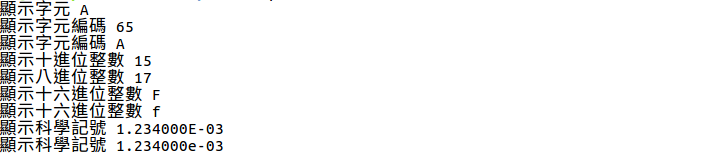
\includegraphics[width=17cm]{fig/cpp_io/HW007}
\end{figure}

\subsubsection {scanf輸入指令}
C語言使用scanf函數從標準輸入(standard input)來讀取變數的值,一般而言,標準輸入指的是鍵盤。scanf的第一個參數是一個字串,通常裡面都放格式指定字元和空白,表示要讀入的變數的型態,後面必須加上與格式指定字元同樣個數及相應型態的變數,並且在變數前要加上\&字元,以下是一個簡單的範例:
\begin{cppcode}
#include <stdio.h>

int main() {
	int input;
	printf("請輸入數字:");
	scanf("%d", &input);
	printf("您輸入的數字:%d\n", input);
	return 0;
}
\end{cppcode}
其執行結果如下:
\begin{figure}[H]
	
\includegraphics[width=17cm]{fig/cpp_io/HW008}
\end{figure}


\subsection{\cc{}語言的輸入和輸出}
\cc{}語言使用cin和cout來做輸入和輸出,使用\cc{}語言的輸入輸出,程式碼必須引入檔頭<iostream>。另外\cc{}有所謂的命名空間,所有標準輸入和輸出相關的函數、指令和參數等,都定義在std的命名空間中,使用這些函數、指令或參數的時候,必須在前面加上std::,例如使用cout的時候,必須寫成std::cout,如果覺得這樣很麻煩,可以在引入檔頭之後,加上以下指令
\begin{inside}
	using namespace std;
\end{inside}
代表要引入std命名空間中的所有函數、指令和參數等,這樣就可以直接使用cout等指令,不用再加上std::的前綴。

以下先介紹cout的用法,接著再介紹cin的用法。

\subsubsection{cout輸出指令}
\cc{}語言使用cout指令將資料送到標準輸出,若沒有特別設定,會由電腦螢幕上顯示。使用方式以範例說明如下:
\begin{inside}
	cout << "String";
	cout << "String" << var1;
	cout << var1 << var2;
\end{inside}
其中\texttt{<<}為輸出運算子,字串與變數會分別以相應的預設格式輸出,不需要使用格式指定字元。例如以下範例程式:
 \begin{cppcode}
 	#include <iostream>
 	using namespace std;
 	int main()
 	{
 		cout<<"Hello world!"<<endl;
 	    cout<<"Hello world!"<<12345<<endl;
 		cout<<12345<<67890<<endl;
 		reurn 0;
 	}
 \end{cppcode}
其輸出結果如下:
 \begin{figure}[H]
 	\centering
	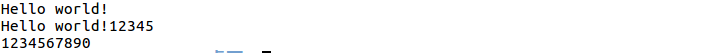
\includegraphics[width=18cm]{fig/cpp_io/HW002}
 \end{figure}
在cout輸出指令中,可以單獨輸出endl符號,代表換行字元,或者也可以使用`$\backslash$n'字元來達到相同的效果。例如以下範例:
\begin{cppcode}
	#include <iostream>
	using namespace std;
	int main()
	{
		int x=20,y=15;
		cout<<"求兩數和\n";  
		//相同於cout<<"求兩數之和"<<endl;
		cout<<x<<"+"<<y<<"="<<x+y<<"\n";
		//相同於cout<<x<<"+"<<y<<"="<<x+y<<endl;
		return 0;
}	
\end{cppcode}
其執行結果如下:
\begin{figure}[H]
\centering
	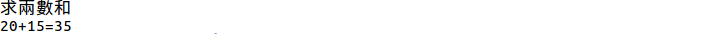
\includegraphics[width=17cm]{fig/cpp_io/HW-003}
\end{figure}


\subsubsection{cin輸入指令}
\cc{}語言使用cin指令從標準輸入讀取資料到相對應的變數中,若沒有特別設定,會由鍵盤輸入讀取,使用者輸入資料後按下【Enter鍵】時,會自動以空白(Space)鍵或Tab鍵作為資料的分隔字元,故輸入之資料不可含空白鍵或Tab鍵。使用方式以範例說明如下:
\begin{inside}
	cin >> var;
	cin >> var1 >> var2;
\end{inside}
分別代表從鍵盤讀取資料到var及var1和var2,其格式依變數型態自動判別。例如以下範例程式:
\begin{cppcode}
//求兩數四則運算
#include <iostream>
using namespace std;
int main()
{
	float x,y;  //宣告 x,y為浮點數
	cout<<"輸入x=";
	cin>>x;
	cout<<"輸入y(不可為0)=";
	cin>>y;
	cout<<"x+y="<<x+y<<endl;
	cout<<"x-y="<<x-y<<endl;
	cout<<"x*y="<<x*y<<endl;
	cout<<"x/y="<<x/y<<endl;	
	system("PAUSE");
	return 0;				
}
\end{cppcode}
其執行結果如下:
\begin{figure}[H]
	\centering
	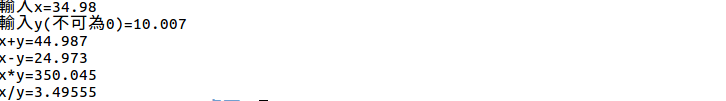
\includegraphics[width=18cm]{fig/cpp_io/HW006}
\end{figure}

